\chapter{Introduction}

This manual is meant to be as complete as possible an introduction to the various hardware features of the \jr. In it, I will attempt to explain each of the major subsystems of the \jr\ and provide simple but practical examples of their use.

One thing this manual will not provide is a tutorial in programming the 65C02 processor at the heart of the \jr. There are plenty of excellent books and videos explaining how the processor works and how to do assembly programming. While examples will generally be written in assembly, I will try to annotate them fully so that what is happening is very clear even to the novice assembly language coder.

Several of chapters in this manual include example assembly code to show how the various features of the \jr\ work. While the code included in the text should be executable, the complete examples can be found on the Github repository that hosts the manual itself. Most of the examples are able to run on their own, but a few of them expect there to be some sort of operating system providing text display routines compatible with the old Commodore kernel. The examples were all written on a machine using OpenKERNAL, which was written for the \jr, but really anything that provides the CINT and CHROUT calls should work fine. Of course, the examples could be tweaked without too much trouble to run on essentially any operating system.

\subsection*{A Note on Notation}

Important side notes are called out with a black bar in the margin. These notes generally call out key differences between the different versions of the \jr\ and may have some important considerations for programs that need to run on all versions.

Example code in this manual is presented as assembly language. While the code is fairly generic 65C02 assembly code, the code was tested using the 64TASS assembler, and there points of 64TASS syntax that are worth explaining.

\begin{itemize}
\item Numeric literals are in decimal unless prefixed by the dollar sign (\$)
\item There are several math and logical operators that can be used to calculate a numeric literal value at assembly time: \verb|+| adds numbers, \verb+-+ subtracts, \verb+*+ multiplies, \verb+|+ calculates the bitwise OR of two values, and \verb+~+ computes the bitwise NOT or negation of a value.
\item The \verb+.byte+ directive stores a set of 8-bit values into the assembled code. The directive takes a list of values puts them into the assembled code as bytes.
\item The \verb+.word+ directive stores a set of 16-bit values into the assembled code. The directive takes a list of values and treats them as 16-bit (even if they are less than 256).
\item There are special operators for selecting specific bit ranges from a number to allow the assembly code to write the number byte-by-byte. The less than character (\verb+<+) selects bits 0--7. The greater than character (\verb+>+) selects bits 8--15. The back tick character (\verb+`+) selects bits 16--23. For example:
\end{itemize}

\begin{verbatim}
    SAMPLE = $123456

    lda #<SAMPLE
    sta $0800           ; Store $56 to $0800
    lda #>SAMPLE
    sta $0801           ; Store $34 to $0801
    lda #`SAMPLE
    sta $0802           ; Store $12 to $0802
\end{verbatim}

\section*{About the Machine}

\subsection*{Ports}

The connectors of the back of the \jr\ from left to right are (see figure:~\ref{fig:rear}):

\begin{description}
    \item[Audio Line Out] the stereo audio output. These are standard RCA style line level outputs.

    \item[SD Card Slot] for standard SD cards for storage of files and programs.

    \item[DVI Monitor Port] for output to your monitor. This can be connected to the DVI input of a monitor or run through a simple DVI-VGA connector to use with an older VGA input.

    \item[IEC Serial Port] supports the Commodore serial bus. A Commodore disk drive (1541, 1571, 1581, {\it etc.}), a Commodore compatible serial printer, or other device supporting the Commodore serial bus can be connected here.
\end{description}

\begin{figure}[ht]
    \begin{center}
        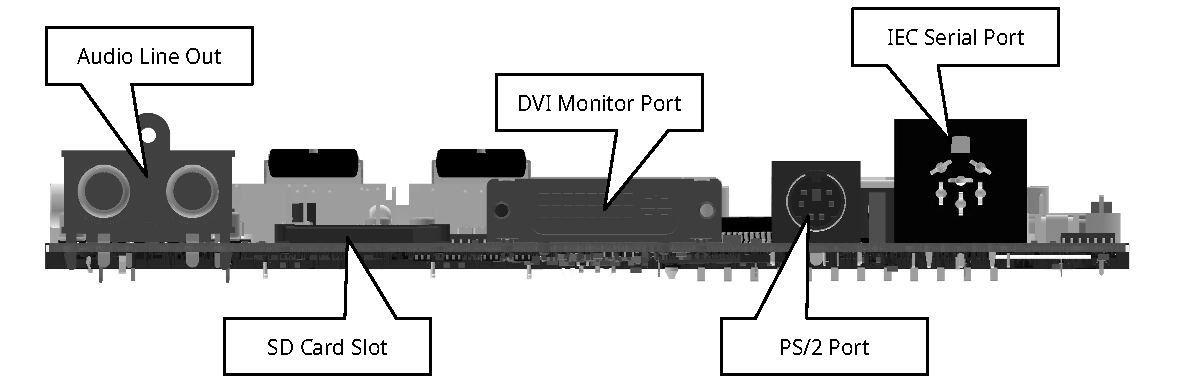
\includegraphics[scale=0.75]{images/f256_render_annotated_back.pdf}
    \end{center}
    \caption{F256jr Rear Connectors}
    \label{fig:rear}
\end{figure}

The top of the board has several connectors and other features that should be explained (see figure:~\ref{fig:top}):

\begin{description}
    \item[Power In] this is a standard ITX/ATX style power connector. Pretty much any PC power supply should work here, and a Pico-ATX style power adapter is more than sufficient.

    \item[Debug USB Port] this provides access to the debug interface of the \jr\ for a desktop computer. You can use it to upload data to the \jr's memory or examine the memory. There is a Mini USB B connector on the board, but there is also a header that can be used to connect the USB jack on some cases to the board.

    \item[Case Buttons and LEDs] this collection of headers is used to connect the power and reset button from the case as well as the power LED and SD access LED.

    \item[Joystick Ports] these connectors allow you to plug in Atari style joysticks

    \item[DIP Switches] these switches allow you to manage certain aspects of the \jr. In particular, you can control gamma correction and some boot options, depending on the kernel installed.

    \item[Stereo SIDs] out of the box, these will be bare sockets, but they are where you would install your SID chips or SID emulators. The sockets support the original 6581, the lower voltage 8581, and the different replacements like the SwinSID, ARMSID, and BackSID.

    \item[Wi-Fi Module] this optional module works with the built-in serial port to allow for Wi-Fi access, if a program or operating system supports it.

    \item[RS-232 Port] this IDC header works with a standard IDC to DB-9 adapter cable to provide an RS-232 serial port. The same serial port is used for this port as is used by the Wi-Fi module, so only one of the two can be used at a time.

    \item[GPIO] this header provides access to the I/O pins of the WDC65C22 VIA. The pin assignments are compatible with the Commodore C64 keyboard connector.

    \item[Expansion Port] for future expansion. This is a PCI-E style connector with a custom pinout. In the future, it might be used for memory expansion or other devices.

    \item[Clock Battery] this CR2032 cell holder provides power for the real time clock chip.

    \item[FPGA JTAG Port] this connector is used to apply any future updates to the FPGA. A special adapter would need to be used to connect to this port.

    \item[Gamepad Ports] this header provides access for an NES or SNES style gameport interface.

    \item[Case Audio Port] this header provides access to the headphone and microphone signals to connect to a PC case.

    \item[Headphone Out] this is a standard headphone adapter port that can be used if the case does not provide headphone output.
\end{description}

\begin{figure}[ht]
    \begin{center}
        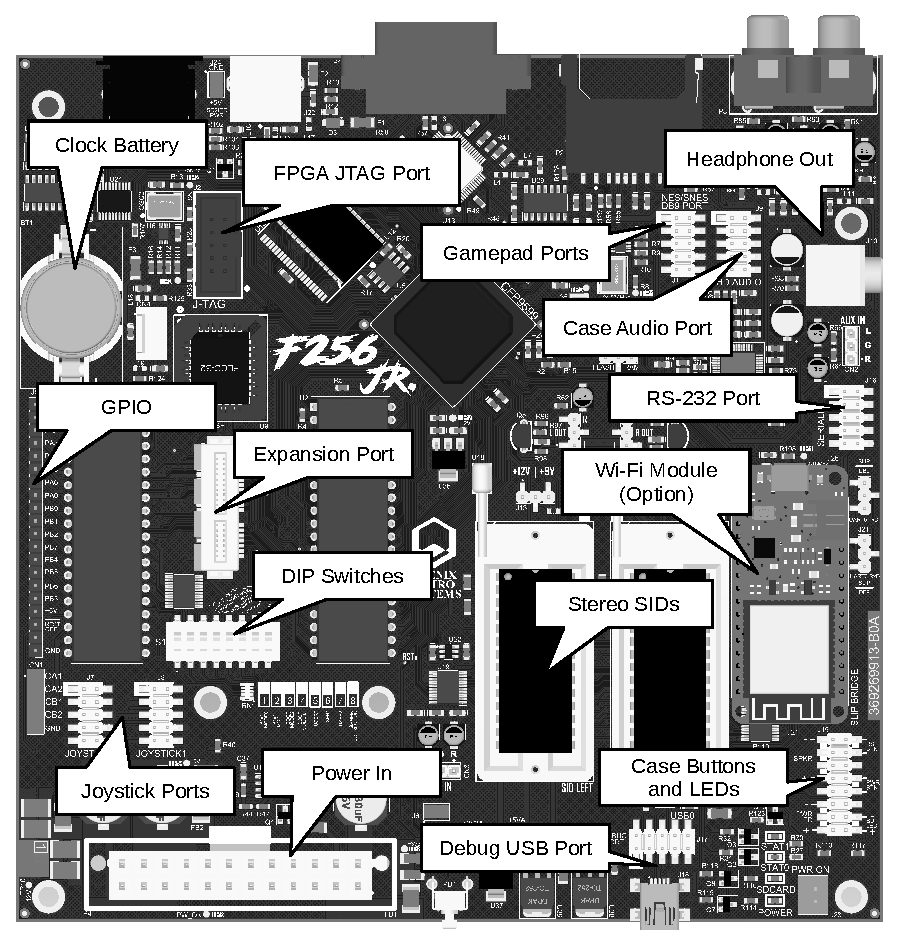
\includegraphics[scale=0.55]{images/f256_render_annotated_top.pdf}
    \end{center}
    \caption{F256jr Top View}
    \label{fig:top}
\end{figure}

\subsection*{System Architecture}

For being so small, the \jr\ has a lot of components to it, so it is worth mapping out the over all structure of the computer. One of the main things to note is that most of what makes the \jr\ the \jr\ is the FPGA TinyVicky. TinyVicky provides the MMU, the various text and graphics engines, most of the I/O devices, controllers for the sound chips, and the controller for the first 256KB of SRAM. The CPU, VIA, RTC, flash memory, and expansion RAM are separate from TinyVicky, although TinyVicky is still responsible for translating CPU addresses to the appropriate chip selection logic and bank selection. One of the most important aspects of this architecture is that, while the first 256KB of SRAM is accessible to both the CPU and TinyVicky, TinyVicky cannot access the data in the flash or in any expansion RAM.

\begin{figure}[ht]
    \begin{center}
        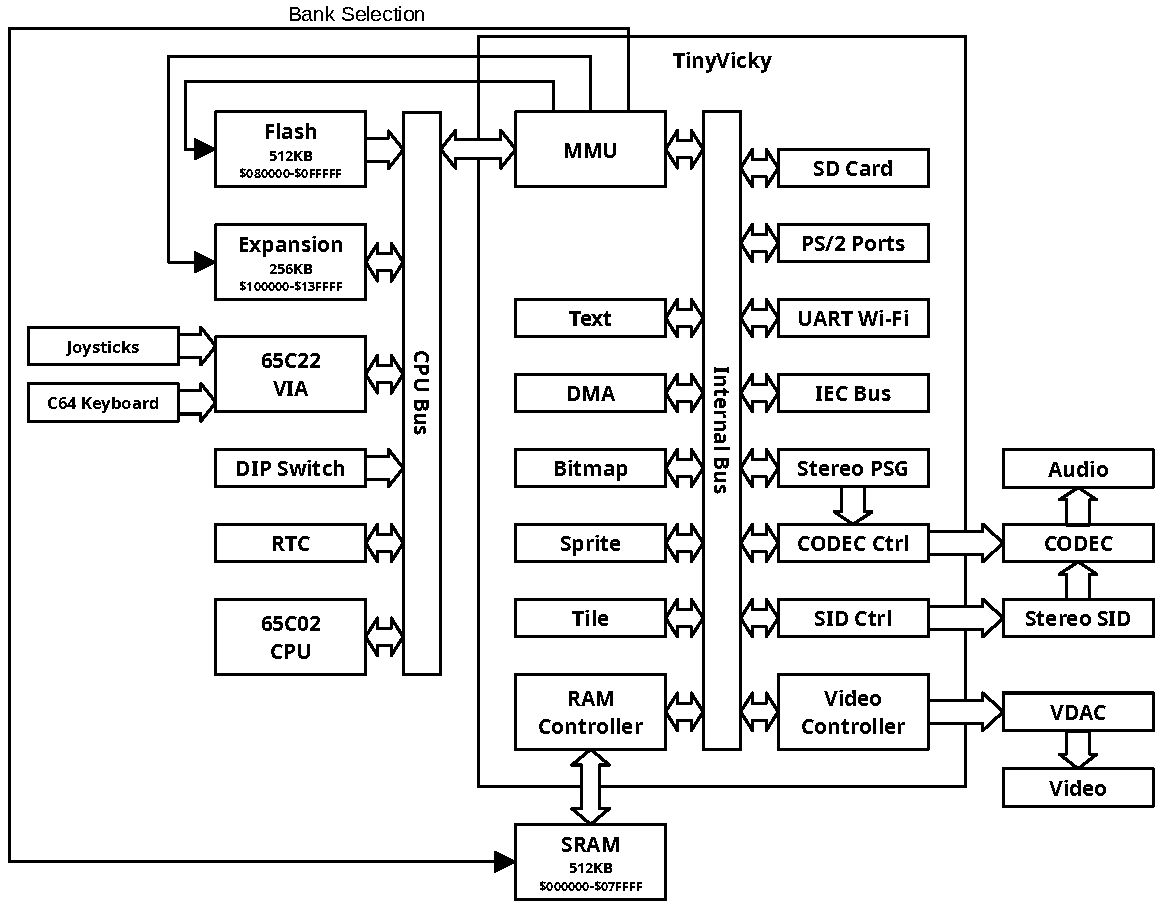
\includegraphics[scale=0.55]{images/f256jr_layout.pdf}
    \end{center}
    \caption{F256jr Internal Architecture}
    \label{fig:arch}
\end{figure}
